\documentclass{article}
\usepackage{graphicx} % Required for inserting images
\graphicspath{ {./images/} }
\usepackage[square,numbers]{natbib}
\usepackage[letterpaper,top=2cm,bottom=2cm,left=3cm,right=3cm,marginparwidth=1.75cm]{geometry}
\usepackage{hyperref}
\usepackage{placeins}

\bibliographystyle{dinat}


\begin{document}


\title{Unit 13}
\author{Chris Hadden}
\date{}
\maketitle

\section{P6 Target Audience for the Pampered Pets Campaign}
Pampered Pets have identified what channels would give them the most impact, and what channels customers also want to use to reach out to brands. From this we now want to focus in on the target audience Pampered Pets should be looking at.

\section{Market Segmentation Analysis}
There are a number of ways of splitting up your target audience and researching what how sections respond to your market area. We will work through this.

\subsection{Age}
It is always worth seeing how your target market may break down by age. 

Looking at SproutSocial's breakdown of social media user age range \cite{sproutage}
\begin{center}
    \begin{tabular}{||c c c c||} 
     \hline
     Age & Top & Middle & Bottom \\ [0.5ex] 
     \hline\hline
     18-29 & Snapchat (41\%) & TikTok (35\%) & Instagram (32\%) \\ 
     \hline
     30-39 & LinkedIn (34\%), & X/Twitter (34\%) & Snapchat (33\%) \\
     \hline
     40-49 & LinkedIn (25\%) & Facebook (22\%) & X/Twitter (21\%) \\
     \hline
     50-59 & Facebook (29\%) & LinkedIn (24\%) & Pinterest (24\%) \\
     \hline
    \end{tabular}
    \label {Age ranges of social media}
    \end{center}

We can see that Facebook covers the majority of people in the age range 40 to 59 and Snapchat covers most people in the age range 18-39. This gives us quite a good place to start.

Another way of looking at age is to see what pets each age range owns. As we can see from figure \ref{fig:pets} from Forbes \cite{ownersage} there isn't a lot in the age differences, which is reassuring in a way, at least there's no specific age range to target and from what we have seen from the social media platforms it seems like there a few that cover most age ranges.

\FloatBarrier
\begin{figure}[ht]
    \caption{Pet Ownership by Pet}
    \centering
    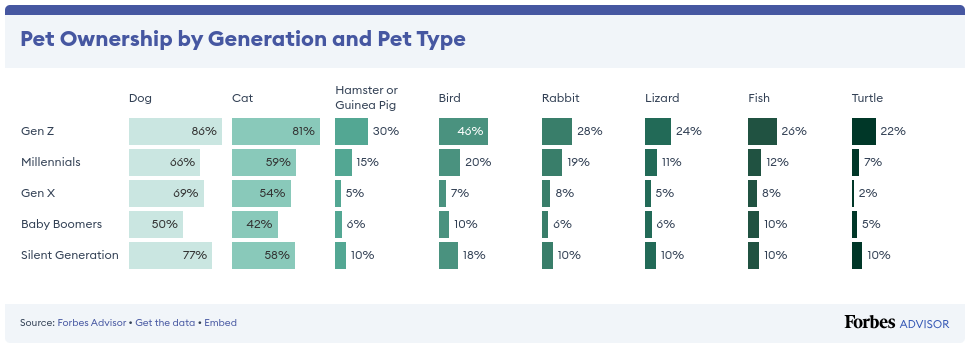
\includegraphics[width=0.8\textwidth]{OwnersByAge}
    \label{fig:pets}
    \end{figure}
    \FloatBarrier

\subsection{Gender}
A study by Inforgroup in America found that "60\% of pet owners are female, 75\% have a household net worth greater than \$220,000, and 77\% are 50 years of age or older ... the analysis also found that more than 58\% of pet owners are college graduates" \cite{data}. This gives us a really good insight in to age, income, gender and education. While this is only one report it does highlight a trend of older more affluent people who are willing to spend more on their pets.

\subsection{Income brackets}
The Inforgroup study \cite{data} has given us a fairly good insight, but we should focus on more specific areas such as income. Income could be a large factor as some people just may not be able to afford much more than the basics and some may have a lot of spare money to spend.
Forbes \cite{forbes} have found that "Households with annual incomes of \$100,000 and over are most likely to own pets: 63\% of households in this income bracket own dogs and 40\% own cats". This lowers the \$220,000 figure we saw previously down to \$100,000.
A different way to look at this was a study from Avma that correlated vet visits and income levels \cite{avma}. They found that "nearly 45\% of respondents in the lowest income category stating that price or affordability is the primary reason they don’t see a veterinarian". They have mentioned a number of outcomes, but one tha may be of interest to Pampered Pets is "A potential approach for expanding access to care is by creating models of veterinary medicine that support a spectrum of care, delivering care at levels other than just the gold standard." This is backed up by Forbes "39.29\% lived on a tighter budget to afford their dogs’ expenses." \cite{forbes}

\subsection{Education}
As stated by \cite{data} the typical owner of a pet will be a college graduate. We can assume that most pet owners will be able to determine what is best for their pets, and that they will be motivated to do so.

\subsection{Geography}
Forbes has data on where most pet owners reside. "Americans in rural areas are more likely to own pets than Americans in suburban and urban areas. 71\% of adults living in rural areas have a pet" \cite{forbes} We may need to consider the types of offers they may suit people in rural areas.

\subsection{Lifestyle}
Certain unexpected lifestyles choices were found by Forbes \cite{forbes}
\begin{itemize}
    \item 13.96\% moved from an apartment to a house so their dog would have a yard.
    \item 7.47\% stayed at a job they disliked because it allowed them to work remotely or had a dog-friendly office.
    \item 6.78\% broke up with a significant other who didn’t like their dog.
    \item 5.25\% took a pay cut or accepted a position with fewer benefits to work remotely or have access to a dog-friendly office.
    \item 4.57\% left a job they liked because another company let them work from home or had a dog-friendly office.
\end{itemize}
We may not be able to do anything about these but it's good to put them in perspective.

\bigskip
\bibliography{bibliography}

\end{document}

